\documentclass[../report.tex]{subfiles}

\begin{document}


\subsection{Transport with a soft target}

\subsubsection{Two-marginal case}

We start with a very simplified approximation of the crowd displacement problem on $\Omega = [0, 1]^2$, with only the first step (with initial agent distribution) and final step decided by the terminal penalty function $G$.

We set $G$ to be the obstacle constraint  related to a subset $\mathscr{O}$ of $\Omega$ as well as a potential $\Psi(x) = d(x, \mathscr A)^{\beta}$ for some $\beta > 0$, related to the distance to a target subset $\mathscr{A}$ (see \cref{fig:CrowdExamplePotential}):
\[
	G(\mu) = \int_\Omega \Psi\,d\mu + \imath_{0}(\mu\mathds{1}_{\mathscr O})
\]
Thus, the agents engage in a one-round mean-field game where they are only concerned with moving to regions with lower potential $\Psi$ -- as close as possible to $\mathscr{A}$ -- whilst obeying physical constraints related to the obstacles.

The discretized MFG problem with viscosity parameter $\epsilon = \sigma^2$ can be written as the following transport problem:
\begin{equation}\label{eq:2MargFuzzyObstacleObj}
\begin{aligned}
	&\inf_\gamma{} \langle \Psi, \gamma^T\mathds{1}\rangle + \epsilon H(\gamma | R_\epsilon) \\
	\suchthat\ & \gamma\mathds{1} = \rho_0, \quad \gamma^T\mathds{1} \odot \mathds{1}_{\mathscr{O}} = 0
	\end{aligned}
\end{equation}
The interesting aspect of this problem is observing what kind of optimal distribution $\rho^*_1 = (\gamma^*)^T\mathds{1}$ the agents reach.

\begin{prop}\label{thm:2MargFuzzyTarget}
Problem \eqref{eq:2MargFuzzyObstacleObj} can be solved in closed form: the Lagrange multiplier $u_0^*$ for the marginal law constraint satisfies
\[
e^{-u_0^*}  = \frac{\rho_0}{R_\epsilon a^*_1}
\]
where $a^*_1 = e^{-\Psi/\epsilon}\odot\mathds{1}_{\Omega\backslash\mathscr{O}}$, and the optimal coupling is
\[
	\gamma^* = R_\epsilon \odot (e^{-u^*}\otimes \hat{\phi})	
\]
It satisfies, as expected, that $\gamma^*_{i,j} = 0$ for all $j\in\mathscr{O}$.
\end{prop}
 
\paragraph{Numerical experiment} We ran a numerical experiment by implementing the solutions given by \cref{thm:2MargFuzzyTarget} to the discrete MFG \eqref{eq:2MargFuzzyObstacleObj}. \cref{fig:2MargFuzzyTransportObstacles} provides a representation of both . We also checked the results when removing the constraints on the obstacles (essentially setting $\mathscr{O}$), and when lowering the viscosity parameter $\sigma = \sqrt{\epsilon}$ (see \cref{fig:2MargFuzzyTransportRelaxedObst,fig:2MargFuzzyTransportLowVisc}).

Of course, replacing $G$ by a hard marginal constraint turns the problem into a classical regularized OT problem, and the above proposition leads to usual Sinkhorn iterations on the grid. The matrix-vector product in the Lagrange multiplier potentially becomes a computational bottleneck, but the separability of the heat kernel $R_\epsilon$ allows for fast computation using simple 1D convolutions.


\begin{figure}
	\centering
	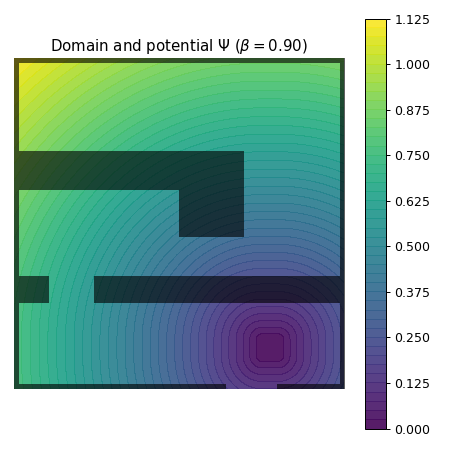
\includegraphics[width=0.5\linewidth]{../project/images/crowd_potential.png}
	\caption{Computational domain of the game $\Omega$ with set of obstacles $\mathscr{O}$ (transparent grey), and contour of the potential function $\Psi(x) = d(x, \mathscr A)^\beta$.} \label{fig:CrowdExamplePotential}	
\end{figure}


\begin{figure}
	\centering
	\begin{subfigure}{.75\linewidth}
	\includegraphics[width=\linewidth]{../project/images/fuzzy_transport_withobstacle.png}
	\caption{Result of the ``fuzzy" transport problem with enforcement of the obstacle constraints and viscosity parameter $\sigma=1$.}\label{fig:2MargFuzzyTransportObstacles}
	\end{subfigure}
	\begin{subfigure}[t]{.38\linewidth}
	\centering
	\includegraphics[width=\linewidth]{../project/images/fuzzy_transport_noobstacle.png}
	\caption{Final distribution $\rho^*_1$ without enforcing the obstacles. The mass of the distribution ``bleeds" through the obstacles. }\label{fig:2MargFuzzyTransportRelaxedObst}
	\end{subfigure}
	\begin{subfigure}[t]{.38\linewidth}
	\centering
	\includegraphics[width=\linewidth]{../project/images/fuzzy_transport_lowvisc.png}
	\caption{Obstacles are constrained as in \cref{fig:2MargFuzzyTransportObstacles}, but with a lower viscosity parameter $\sigma=0.4$.}\label{fig:2MargFuzzyTransportLowVisc}
	\end{subfigure}
	\caption{Marginal distributions of the solution of two-step MFG or ``fuzzy transport" problem \eqref{eq:2MargFuzzyObstacleObj}, with a few variations.}\label{fig:2MargFuzzyTransportMarginals}
\end{figure}



\begin{remark}[A ``smarter" (more realistic) potential for crowd dynamics]\label{rmk:SmartPotential} The results shown \cref{fig:2MargFuzzyTransportMarginals} are satisfactory for the given potential $\Psi$ -- as expected the agents try to stay near the low-potential regions. However, for modeling of crowd dynamics they would be deeply nonphysical because the potential is inadequate. In a room evacuation scenario, for instance, agents would seek to minimize the time-to-exit: the literature shows this leads to the Eikonal equation, a kind of Hamilton-Jacobi PDE. We computed the adequate potential shown \cref{fig:CrowdShortedPathPotential} using the Fast Sweeping method \parencite{Zhao2004AFS}, as well as the discrete MFG \cref{fig:2MargEikonalGame}.
\end{remark}


\begin{figure}
	\centering
	\begin{subfigure}[t]{.4\linewidth}
		\centering
		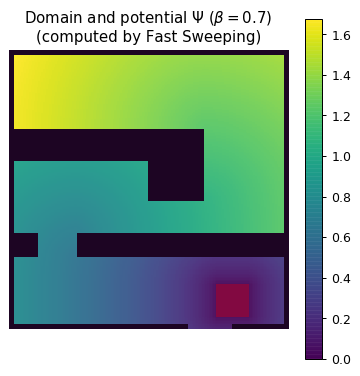
\includegraphics[width=\linewidth]{../project/images/crowd_eikonal_potential.png}
		\caption{Domain and potential associated with the fastest path distance.}\label{fig:CrowdShortedPathPotential}
	\end{subfigure}
	\begin{subfigure}[t]{.4\linewidth}
		\centering
		\includegraphics[width=\linewidth]{../project/images/eikonal_transport_lowvisc.png}
		\caption{Optimal terminal distribution $\rho^*_1$ of the discrete MFG with the potential from \cref{fig:CrowdShortedPathPotential}.}\label{fig:2MargEikonalGame}
	\end{subfigure}
	\caption{Setup and solution for the discrete MFG using the time-to-exit potential discussed in \cref{rmk:SmartPotential}.}
\end{figure}

\subsubsection{One intermediate time step}

We now go up to three marginals $(\rho_0,\rho_1,\rho_2)$. We assign to the single intermediate marginal $\rho_1$ the congestion constraint $\rho_1 \leq \bar{m}$ and the obstacle constraint. The primal problem then reads
\begin{equation}
\begin{aligned}
	&\inf_{\gamma,\rho_1,\rho_2}{} \langle \Psi, \rho_2\rangle + \epsilon H(\gamma | R_\epsilon) \\
	\suchthat \ & P^k_\#\gamma = \rho_k,\; k = 1,2 \\
	& \rho_1 \leq \bar{m} \\
	& \rho_1\odot\mathds{1}_{\mathscr O} = 0\\
	& \rho_2\odot\mathds{1}_{\mathscr O} = 0
\end{aligned}
\end{equation}

\begin{prop}
The Lagrange multipliers $u_i^*$ at the optimum satisfy the fixed-point conditions:
\begin{align*}
	&a_0^* = \frac{\rho_0}{R_\epsilon[\cdot, a_1^*, a_2^*]} \\
	&a_1^* = \min\left(\frac{\bar{m}}{R_\epsilon[a_0^*,\cdot,a_1^*]}\right)
\end{align*}
where $a_i^* = \exp(-u_i^*)$, $a_1^*$ is supported on $\Omega\backslash\mathscr{O}$ and $a_2^* = e^{-\Psi/\epsilon}\odot\mathds{1}_{\Omega\backslash\mathscr{O}}$, and we denote $R_\epsilon[\cdot,\cdot,\cdot]$ the tensor product by $R_\epsilon$.
\end{prop}

The fixed point can then computed using an iterative algorithm à la generalized Sinkhorn, just as in the Algorithm \autoref{algo:Algo1} suggested by \cite{benamou2018entropy}.

The issue of computational efficiency is more pronounced here than before due to the tensor product and need for multiple iterations until convergence.


\end{document}
